		We here introduce the model of Butt\`a, Flandoli, Ottobre and Zegarlinski \cite{Butta2019}. This is a Vicsek-type continuum model for an interacting particle system. There are three key parts to this model that together create interaction and ordered motion: a herding function, denoted $G$; an averaging function, denoted $M$; and an interaction function, $\phi$. Each will be described before the full model is introduced. Throughout, we will be considering the phase space distribution function $f_t(x,v)$, where $(x,v) \in \T \times \R$ and $t \in \R$ with $\T \cong \R \backslash \Z \cong S^1$ denoting the unit one-dimensional torus. The distribution function represents the density of particles at time $t$ at a given point in phase space $(x,v)$.
		
		The interaction function, $\phi: \T \to \R $ acts on the smallest scale, between individual points. It is smooth and satisfies the following:
		\begin{align}\label{eq:phi}
			\phi(x) \geq \epsilon >0, && \phi(x) = \phi(-x), &&& \int_{\T} \phi(x) \dif x = 1.
		\end{align}
		These are quite natural ways to describe an interaction. The first means that all points interact with each other to some degree. The second requires symmetry when interacting, and finally the function must have unit integral -- this is only for simplicity and could in fact be any value, so long as it is finite. For example, we may take $\phi \equiv 1$. This will satisfy the above requirements and corresponds to all points interacting an equal amount, regardless of position on the torus. This will create space-homogeneity, which we will return to later.
		
		The function $M:\R \to \R$ takes a weighted average of the interactions across the space.	
		\[ 
			M(t,x) = \frac{\int_{\T}\int_{\R}f_t(y,w)\phi(x-y)w\dif w \dif y}{\int_{\T}\int_{\R}f_t(y,w)\phi(x-y)\dif w \dif y}
		\]
		The interaction function provides the weighting. Note the argument of  $\phi$ is the distance between two points in space and also that $M$ depends on $f_t$. The denominator is required in the corresponding particle model to prevent the size of the group of particles from having an effect on the dynamics. It can be thought of as a normaliser.
		
		Finally, the herding function $G:\R \to \R$ is chosen such that
		\begin{align*}
			&G(u)=-G(-u),&& {\begin{cases}
								G(u)>u & \text{ if } 0< u <1\\
								G(u)<u & \text{ if } u > 1
				   		   \end{cases}}.
		\end{align*}
		We shall consider three forms of $G$.
		\begin{enumerate}
			\item Step:
			\[
				G(u) = \frac{1+\beta \mathrm{sgn}(u)}{1+\beta}, \qquad \beta > 0	
			\]
			This is the usual choice in the biological literature, with \(\beta = \frac{1}{2}\). It is differentiable everywhere with $G'(u) = \frac{1}{1+\beta}$, except at $u=0$. This discontinuity makes analysis more difficult.
			\item Smooth:
			\[
				G(u) = \frac{\arctan(u)}{\arctan(1)}
			\]
			Here we get a much smoother curve that is everywhere differentiable. However the gradient isn't very steep and there is no way to control the shape of the curve.
			\item Sigmoid:
			\[
				G(u) = \frac{2}{1+\mathrm{e}^{-\alpha u}} - 1 , \qquad \alpha >0
			\]
			The sigmoid herding function provides a middle ground between the previous two. It is smooth, but can be made as sharp as required by adjusting the parameter $\alpha$. However note that it only satisfies second requirement above in the limit as $\alpha \to \infty$ as the function is bounded above by 1.
		\end{enumerate}
		During the analysis, we will use the smooth herding function for its amenability. The role of $G$ is to herd the mean velocity towards a fixed value -- in this case plus or minus one. How it does so will become clearer when we discuss the dynamics of the model.
        \begin{figure}
            \centering
            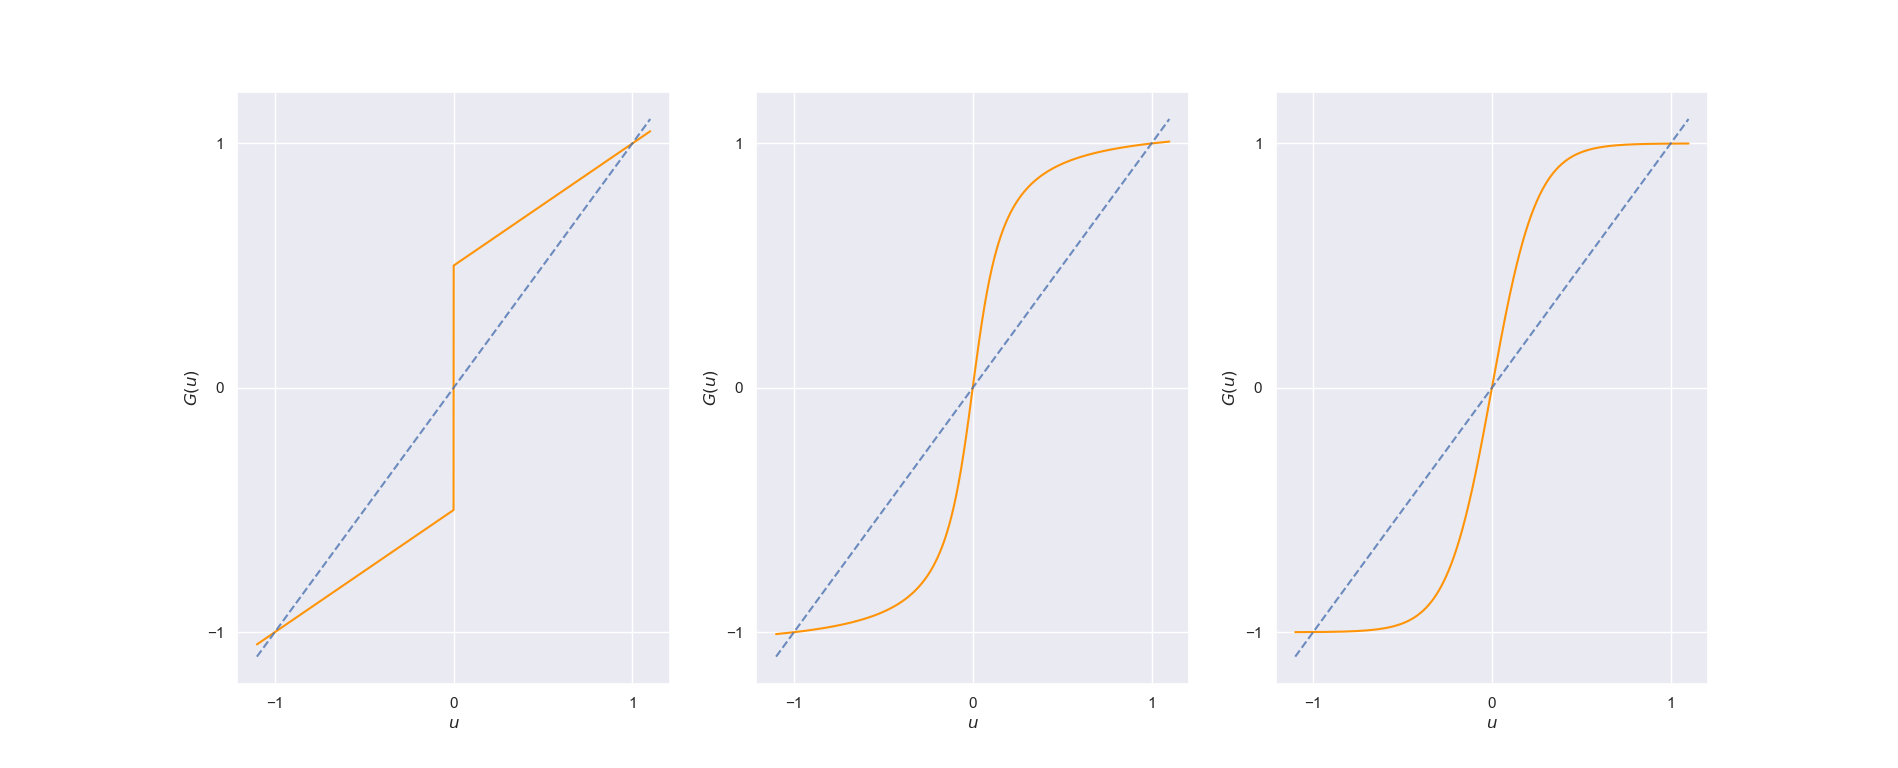
\includegraphics[width=\linewidth]{Figures/herdingfunctions}
            \caption{Step, smooth and sigmoid herding functions, with the dashed line $y=x$ for reference}
            \label{fig:herdingfunctions}
        \end{figure}
		We now have all the necessary ingredients to give the full continuum model. The evolution of the distribution is described by
		\begin{equation}\label{eq:fullPDE}
			\partial_t f_t(x,v) = -v\partial_x f_t(x,v)  +\partial_v v f_t(x,v) - \partial_v \left[ G(M(t,x))f_t(x,v)\right] + \sigma \partial_{vv}f_t(x,v),
		\end{equation}
		where $\sigma > 0$ is a constant describing the rate of diffusion. At its heart, this is just an advection-diffusion equation. The first term illustrates the movement around the torus, the second describes a damping effect and the fourth gives a diffusive effect in velocity. The third term is where the interest lies as it contains all the information on interaction and herding.
		